\chapter{Forschungsmethodik}
Als Forschungsmethode wird in dieser Arbeit der \hcdp{} nach \citet{Norman13} angewandt.
Diese Forschungsmethode wurde gewählt, da die Entwicklung nah am Anwender stattfindet und es sich um einen agilen Softwareentwicklungsprozess\urlnote{https://www.it-agile.de/wissen/einstieg-und-ueberblick/was-ist-agile-produktentwicklung/}{22.11.2017} handelt.
Zudem ist die Usability der entwickelten App wichtig, da die Endanwender nicht IT-affin sind und die Aufmaßerfassung auf einem kleinen Smartphone-Display schwierig ist. \\

\noindent
\citeauthor{Norman13} selbst definiert den Prozess in seinem Buch ``The Design of Everyday Things: Revised and Expanded Version'' wie folgt \citep[Abbildung 6.2]{Norman13}:

\begin{quote}
  ``Make observations on the intended target population, generate ideas, produce prototypes and test them.
  Repeat until satisfied.''
\end{quote}

\noindent
Die Idee des \hcdp{} ist es, eine ausgewählte Menge an Testpersonen aus der Zielgruppe in ihrem Alltag zu beobachten.
Hierbei sollen mögliche Usability-Probleme identifiziert werden.
Anschließend sollen diese Usability-Probleme durch das Entwickeln verschiedener Ideen und eines Prototyps gelöst werden.
Diesbezüglich beschreibt \citeauthor{Norman13} den Prozess als Zyklus (siehe \autoref{fig:hcp}), welcher sich aus vier verschiedenen Phasen zusammensetzt:

\begin{enumerate}
  \item Observation (Beobachtung) \label{itm:observation}
  \item Idea Generation (Ideenfindung) \label{itm:idea}
  \item Prototyping (Entwicklung eines Prototyps) \label{itm:prototyping}
  \item Testing (Testen) \label{itm:testing}
\end{enumerate}

\begin{figure}[h]
  \centering
  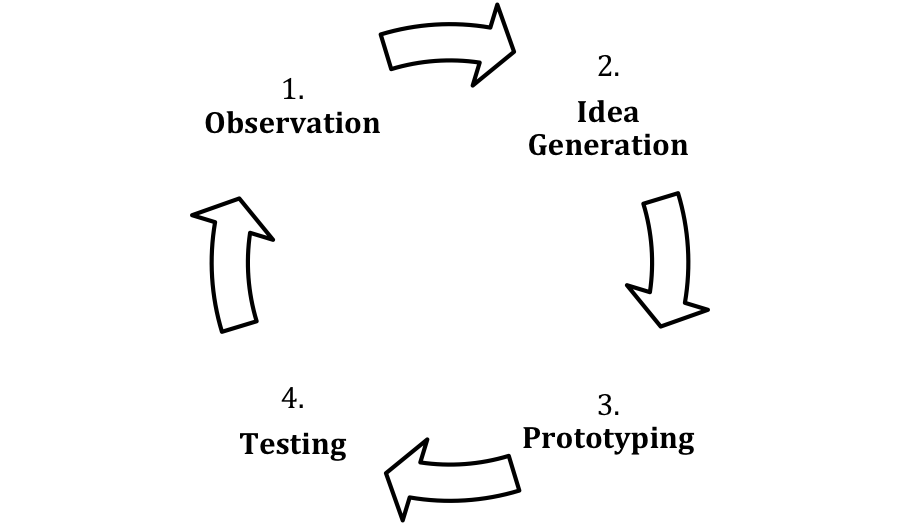
\includegraphics[keepaspectratio]{hcp}
  \src{http://www.adampatrickbell.com/blog/makey-makey-instrument-invention-part-iii-constrain-to-create}{15.01.2018}
  \caption{The Human-Centered Design Process}
  \label{fig:hcp}
\end{figure}

\noindent
Dieser Zyklus wird iterativ so lange wiederholt, bis sich in der Testphase keine weiteren Usability-Probleme mehr identifizieren lassen oder man mit den bis dahin erzielten Ergebnissen zufrieden ist. \\

In der ersten Phase des Zyklus (\emph{Observation}) wird eine Menge an ausgewählten Testpersonen bei der Bearbeitung von Aufgaben beobachtet, die für das zu untersuchende Problemgebiet relevant sind.
Hierbei werden alle auftretenden Probleme notiert, und auf ihre eventuellen Ursachen untersucht.
Auf diese Weise ist es den Beobachtern möglich, ein tiefgründiges Verständnis für die angestrebten Ziele und den dabei anfallenden Problemen der Testpersonen zu erlangen.
Bezogen auf diese Arbeit findet die Phase der \emph{Observation} in Kapitel 3 und 4 statt. \\

In der zweiten Phase (\emph{Idea Generation}) werden Lösungsansätze zu den in der ersten Phase identifizierten Problemen aufgestellt.
Hierzu führt \citeauthor{Norman13} drei Richtlinien zur Orientierung an \citep[Seite 226]{Norman13}:

\begin{itemize}
  \item ``Generate numerous ideas'' (Generiere viele Ideen)
  \item ``Be creative without regard for constraints'' (Sei grenzenlos kreativ)
  \item ``Question everything'' (Hinterfrage alles)
\end{itemize}

\noindent
Zusammengefasst sagen diese drei Regeln aus, dass es während der \emph{Idea Generation} sinnvoll sei, viele kreative Lösungsansätze für die Usability-Probleme aufzustellen und zu hinterfragen.
Nach \citeauthor{Norman13} könne selbst eine anfangs nicht viel versprechende Idee zur Findung der finalen Lösung einen kleinen Anteil beitragen.
Die Phase der \emph{Idea Generation} findet in Kapitel 5, bei der Konzeption der eigenen App, statt. \\

Anschließend werden die Lösungsansätze in der dritten Phase (\emph{Prototyping}) in Form eines Prototyps umgesetzt.
Diese Phase korrespondiert zu Kapitel 6.1 dieser Arbeit. \\

In der vierten Phase des Zyklus (\emph{Testing}) wird der entwickelte Prototyp an ausgewählte Testpersonen verteilt.
Bei der Auswertung der Testergebnisse soll geprüft werden, ob die in Phase 1 identifizierten Probleme gelöst werden konnten.
Sollten keine weiteren Usability-Probleme während des \emph{Testing} auftreten, kann der \hcdp{} an dieser Stelle erfolgreich beendet werden.
Kommt es jedoch dazu, dass einzelne Probleme nicht optimal gelöst werden konnten oder neue Probleme identifiziert worden sind, wird eine weitere Iteration des Zyklus mit Hilfe der gewonnenen Testergebnisse gestartet.
Das Kapitel 6.2 beschreibt diese \emph{Testing} Phase.
Anschließend werden in den darauffolgenden Kapiteln 7, 8 und 9 drei weitere Iterationen beschrieben, die nötig sind um einen optimalen Prototyp zu entwickeln.
